\documentclass[dvipdfmx]{jsarticle}
\usepackage[dvipdfmx]{graphicx}
\usepackage{amsmath, amssymb}
\usepackage{mathtools}
\usepackage{here}
\usepackage{caption}
\begin{document}
\title{週間進捗報告}
\author{権藤陸}
\maketitle
\section{進捗}
\begin{itemize}
    \item 論文のサーベイを行いました.以下にカテゴリを示します.
    \begin{itemize}
        \item 点群に基づく人間のidentification
        \item 心拍に基づく人間のidentification
        \item 呼吸に基づく人間のidentification
        \item 歩行特徴に基づく人間のidentification
        \item 人間の行動のclassification
    \end{itemize}
\end{itemize}

\section{各論文の概要}
\subsection{点群に基づく人間のidentification}
\begin{itemize}
    \item 『Human tracking and identification through a millimeter wave radar\cite{pointcloud}』
\end{itemize}

\subsubsection{提案法}
ミリ波レーダ(FMCWレーダ)により,対象となる複数人物の点群を取得し,その点群を追跡することで人間の識別を行っています.システム全体の流れを図1に示します.本研究のモデルは2つの目的があります.1つ目は,12名の被験者の識別.2つ目の目的は,12名の被験者で分類器をトレーニングし,その後テストでトレーニングセットにいない4名の侵入者を検出することです.

\begin{figure}[H]
    \begin{center}
    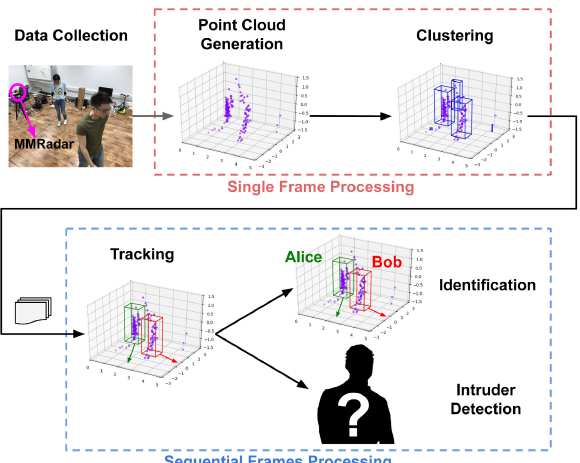
\includegraphics[width=0.7\linewidth]{./img/tuiseki_system.png}
    \end{center}
    \caption{システム概要}
    \end{figure}

\begin{enumerate}
    \item 点群の生成

レーダで取得したデータに対して,range-FFTを行い,対象人物までの距離を計算をした後,静的物体によるクラッタを除去するため,各フレーム内のチャープ全体で,アンテナごとの各レンジビンの平均を減算します.そして,doppler-FFT, angle-FFTを行った後,点群が生成されます.
    \item クラスタリング
    
検出された点群のすべてが人間の動きによるものでは限らないため,DBScanを行い,点をクラスターにマージします.クラスターの数を事前に指定しなくて良いため,監視対象となるシーン内に入ってきたりフェードアウトしていく場合に対応できるメリットがあり,さらにノイズに対処するため,異常値を自動的にマーク可能である.以上の2工程が1つのフレームに対する処理である.
    \item トラッキング
    
トラッキングでは,Hungarian Algorithmを用いて,フレーム間のオブジェクトの関連付けを行います.連続するフレームでトラッキング中のオブジェクトが検出されない場合,そのオブジェクトを非アクティブとしてマークし,その後の対象から外します.その後,x軸とy軸に沿った位置と速度で構成される状態に対し,カルマンフィルタを適用することでトラッキングの修正を行います.
    \item identification
    
identificationでは,軌跡の各フレームから固定サイズのバウンディングボックスを使用し,それをボクセル化し,占有グリッドを形成します.使用されるトラックレット(T枚の占有グリッドを示す?)はスライディングウィンドウ方式でセグメント化されており,各ウィンドウには前のウィンドウとのオーバーラップ率が75\%の2秒間の連続占有グリッドが含まれます.これらの占有グリッドは,Flatten Layerで平坦化されたのちに,Bi-LSTMへ入力されます.使用されるネットワークのアーキテクチャは図2のようになります.Bi-LSTMからの出力は全結合層へ入力され,侵入者検知を行わない場合は,図2の左側のソフトマックスレイヤーに入力され,最終的な分類結果を出力します.

\begin{figure}[H]
    \begin{center}
    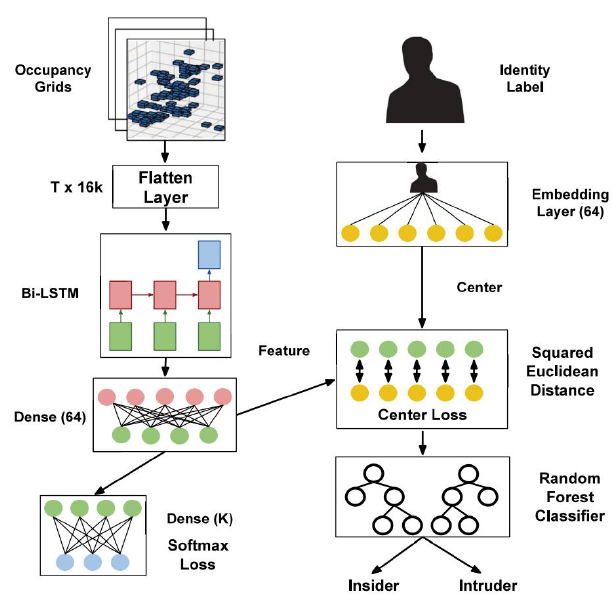
\includegraphics[width=0.6\linewidth]{./img/network_architecture.png}
    \end{center}
    \caption{softmax-lossとcenter-lossでトレーニングされた分類ネットワーク}
\end{figure}

侵入者検知を行う場合には,ソフトマックスレイヤーに加えて,図2右側のセンターロスも学習に用いられます.$L$を損失関数として,$\lambda$で重み付けされたセンターロスが加えられています.

\begin{equation}
L = L_{softmax} + \lambda L_{center}
\end{equation}

センターロスは次のように定義されています.$f_i$は$i$番目の特徴量を表し,$C_{y_i}$はラベル$y$の$i$番目の特徴の中心を表します.

\begin{equation}\label{}
L_{center} = \sum_{i=1}^{m} ||f_i - C_{y_i}||_2^2
\end{equation}

侵入者検知の際には,Embeddingレイヤーを使用して,IDラベルを特徴の中心にマッピングします.侵入者からの特徴は異なる空間分布を持っているため,それぞれから各クラスの中心までの距離が異なります.各クラスの中心までの距離を使用し,ランダムフォレスト分類器を用いてサンプルが侵入者からのものかどうか2値の出力を行います.

\end{enumerate}

\subsubsection{実験諸元と結果}
提案法の評価のために用いられたデータセットは,28人の被験者からデータを収集し,それぞれが指定されたエリアを10分間ランダムに歩く設定としました.年齢は18歳から35歳までで,そのうち13名が女性です.身長は155cmから188cm,体重は48kgから80kgです.また使用されたレーダはIWR1443Boostで3×4のMIMOアンテナアレイを備えています.レーダの使用可能範囲は30mですが,本実験では最大範囲を5mと定めています.
\begin{itemize}
    \item 12名の被験者の識別
    
上で述べた28名の被験者のうち12名分のデータを用いて識別評価を行いました.11:1の比率でトレーニングセットとテストセットに分割しました.12人の被験者の混同行列は図3のようになります.
\begin{figure}[H]
\begin{center}
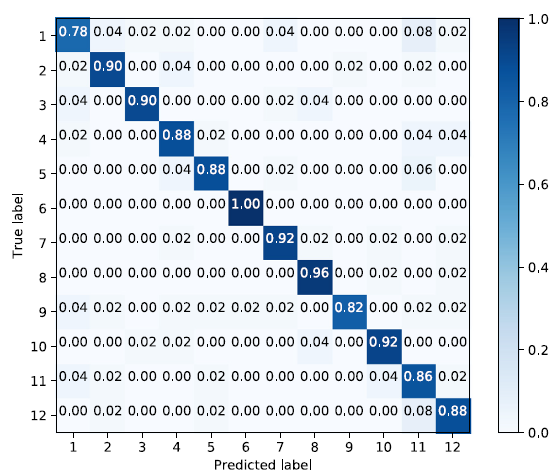
\includegraphics[width=0.6\linewidth]{./img/mID_conf.png}
\end{center}
\caption{12人の被験者の混同行列}
\end{figure}

    \item 侵入者検知

    12名の被験者の識別に用いなかった16名の被験者のデータのうち,12名を内部関係者,4名を侵入者と定義して,侵入者検知を行いました.内部関係者と侵入者のサンプル数の比率は1:1です.内部関係者の人数を変えながら評価を行い,結果は表1のようになりました.内部関係者(Insiders)の人数が増えるごとに,検出精度が劣化していることが確認できます.

\begin{figure}[H]
\caption*{表1: 侵入者検出の精度,再現率,F1スコア}
\begin{center}
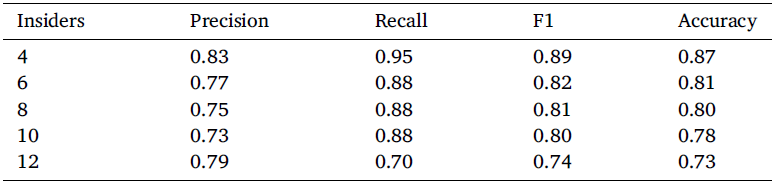
\includegraphics[width=0.8\linewidth]{./img/mID_table.png}
\end{center}
\end{figure}
\end{itemize}

\subsubsection{まとめ}
本論文は点群に対してトラッキングと識別を組み合わせた手法を提案しました.12人の識別では89\%の精度,侵入者検知では,関係者が12人,侵入者が4人の設定で73\%の精度を達成しました.
レーダは家具や壁の中に隠すことが可能であり,カメラのようにプライバシーが保護されないということもありません.そのため,将来的にスマートホームの仕組みの中に導入できる可能性を秘めています.

\subsection{心拍に基づく人間のidentification}
\begin{itemize}
    \item 『Heart signatures: Open-set person identification based on cardiac radar signals\cite{DDLM}』
\end{itemize}

\subsubsection{提案法}

本論文は,レーダベースの心拍信号が,ECG信号の本質的な性質を反映した信号であることを利用し,1D-CNNで特徴量を抽出し,電極に似た概念である双極子を導入し,特徴量+負の双極子と正の双極子が敵対的に学習を進めることでオープンセットにおいても高い精度を達成している.提案されたモデルは,DDLM(Dipole Deep Learning Model)と呼称されます.図4にDDLMのフレームワークを示します.まず,図4中のDDLMについて詳説します.

\begin{figure}[H]
\begin{center}
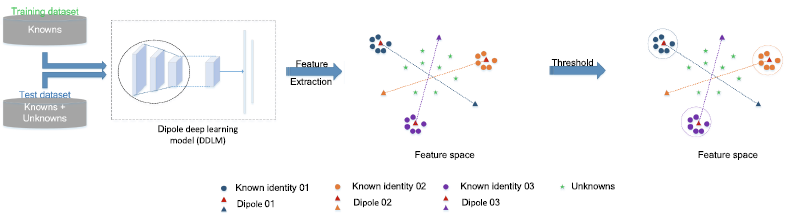
\includegraphics[width=\linewidth]{./img/ddlm_framework.png}
\end{center}
\caption{オープンセット仮定の下での心拍個人識別のためのDDLM法のフレームワーク}
\end{figure}

\begin{itemize}
    \item モデルのアーキテクチャ

DDLMは,図5で表されるような構造になっています.まずは,1D-CNNにデータを入力し,特徴量を抽出します.ここで入力は1つの心拍セグメント$(x, y)$であり,抽出された潜在表現は,学習可能なパラメータ$\theta$を用いて$f\theta (x)$と表されます.$y$はセグメントに対応するアイデンティティを表します.そして,ここで潜在空間での線形分類におけるSoftMaxレイヤー固有の欠陥を改善するため,負極と正極の2つの極で構成される双極子が提案されます.双極子は各クラスの潜在空間に設定され,距離ベースの類似性を分類に適用します.双極子は$m_{ij}$と表され,$i \in {1, ..., n}$で,$n$はクラス数,$j \in {N, P}$は各クラスの負極(Negative)と正極(Positive)のインデックスを表します.
$f\theta (x)と双極子m_{ij}$は,心拍セグメントを入力することでと共にトレーニングされ,モデルは図4の右半分で示されるように,最も近い負の双極子と最も遠い正の双極子を検出します.そして,ユークリッド距離に従い,特定のインスタンスを検出された双極子に割り当てます.

\begin{figure}[H]
    \begin{center}
    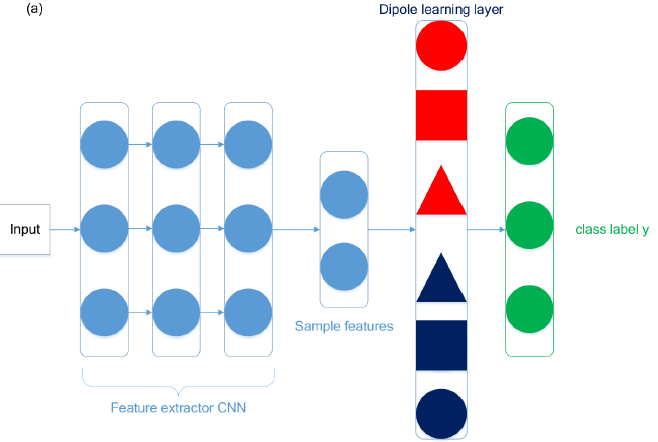
\includegraphics[width=0.8\linewidth]{./img/ddlm_model.png}
    \end{center}
    \caption{DDLMのアーキテクチャ図解}
\end{figure}

    \item 損失関数

本フレームワークでは,モデルは距離を計算し,サンプルの潜在的な特徴と双極子間の類似性を定量化します.ここでは,ユークリッド距離を用いて,サンプル$(x, y)$が属する双極子$m_{ij}$の確率を算出します.

負極では,距離が短い距離であればあるほどよく,正規化された$p(y|x)$を次のように計算します.

\begin{equation}\label{}
p(y|x) = \frac{e^{-\gamma d (f_{\theta (x)}, m_{iN})}}{\sum_{k=1}^{n} e^{-\gamma d (f_{\theta (x)}, m_{kN})}}
\end{equation}

ただし,$d(f_{\theta (x), m_{iN}}) = ||f_{\theta}(x) - m_{iN}||_{2}^{2}$で,$f_{\theta (x)}$から$m_{iN}$までのユークリッド距離を表しています.$\gamma$は各クラスの確率を調整するために使用さっるハイパーパラメータです.$p(y|x)$に基づいて,分類損失は具体的に次のように表されます.

\begin{equation}\label{}
l_{cN}((x, y);\theta, N) = -\log p(y|x)
\end{equation}

正極についても同様の計算が行われますが,正極の場合,潜在空間の特徴量との距離が大きくなるように損失関数がデザインされます.

    \item 正則化

open space riskを軽減するため,負極・正極のどちらにも正則化項を導入します.
負極の正則化項は次のように表されます.

\begin{equation}\label{}
l_{oN}((x, y);\theta, N, S) = ||d(f_{\theta(x), m_{yN}}) - s_y||_{2}^2
\end{equation}
ここで,$m_{yN}$は,ラベル$y$における$f_{\theta}(x)$が所属する負極,$s_y$は学習可能な,負極の範囲を表すパラメータです.この項を導入することにより,ID yに属するサンプルは,負極$m_{yN}$を中心とした範囲$s_y$を持つ球状の空間に拘束されます.$N$については具体的な説明が見つかりませんでしたが,後ほど示すように学習対象の負極パラメータのため,おそらく負極の座標のことを指しているものと考えています.
そして,負極に対する全体の損失は,次のように計算されます.

\begin{equation}\label{}
l_N = l_{cN}((x, y);\theta, N) + \lambda_{0} l_{oN}((x, y);\theta, N, S)
\end{equation}
ただし,$\lambda_{0}$は負極のopen space riskを支配するハイパーパラメータです.

分類損失と同様に,正極の正則化項に関しても,負極と同様に計算されます.

    \item 学習プロセス
敵対的学習において,GAN(Generative Adversarial Network)と異なり,本フレームワークでは,新しいサンプルを生成することなく,双極子自身が敵対者の役割を果たしている.学習プロセスは,$f\theta, N, P$の3者によるminmax gameとみなすことができる.

\begin{equation}\label{}
\underset{f_{\theta,N}}{\min} \underset{P}{\max} (f_{\theta}, N, P)
\end{equation}

具体的なアルゴリズムは以下のようになる.
\begin{figure}[H]
\begin{center}
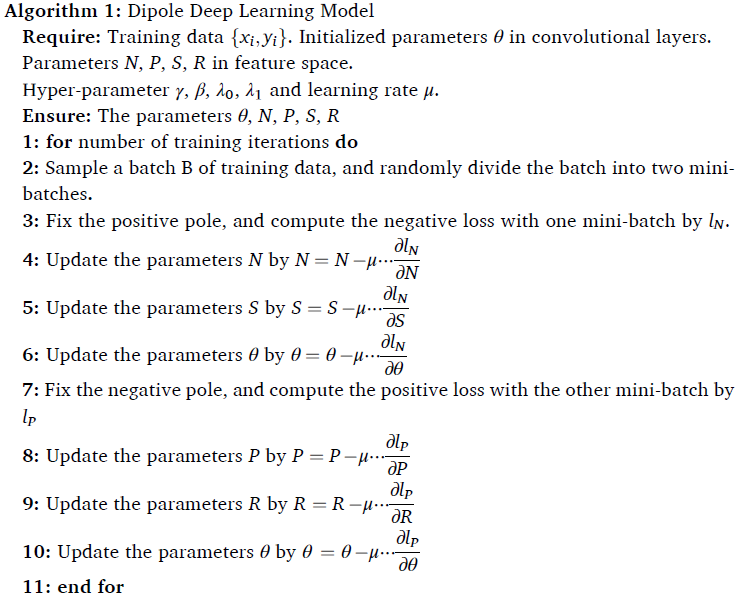
\includegraphics[width=0.8\linewidth]{./img/ddlm_procedure.png}
\end{center}
\end{figure}
\end{itemize}

\subsubsection{実験諸元と結果}
\begin{itemize}
    \item 実験諸元
\end{itemize}
表2に,データセットの概要を示します.

\begin{figure}[H]
\caption*{表2: データセットの概要}
\begin{center}
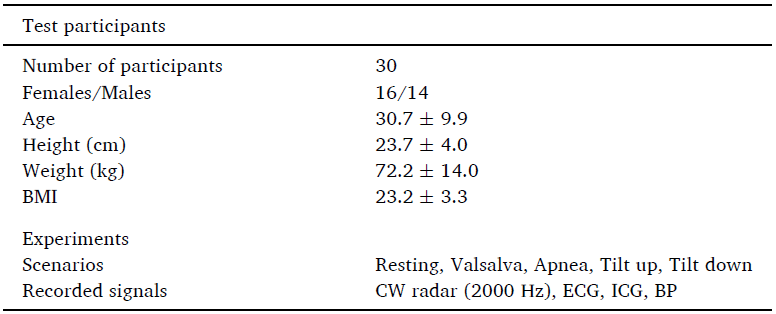
\includegraphics[width=0.7\linewidth]{./img/ddlm_dataset.png}
\end{center}
\end{figure}

本論文では,10分間横になり休息するシナリオで測定されたデータのみが使用されました.また,MATLABで記述された,生データからレーダによる心拍パターンを再構築する公開コードを利用し,250Hzにダウンサンプリングしました.次に,継続的な心拍信号を固定ウィンドウサイズの短いセグメントに分割しました.今回はリアルタイム性と信頼性のトレードオフとして,最適な秒数として(実験の結果)5秒が選択されました.被験者信号の合計時間は600秒で,セグメント間のオーバーラップは1.5秒となっています.1人あたり,172のインスタンスが含まれ,計5160のインスタンスがトレーニングとテストに3:1の比率でランダムに分割されました.各インスタンスはMin-Max正規化によって正規化されています.

オープンセットという条件のため,30人の被験者のうち,15人の心拍信号のみを用いてトレーニングを行い,テストでは30人の信号を用いて検証を行った.また,ここでopenness indexを定義する.

\begin{equation}\label{}
openness = 1 - \sqrt{\frac{C_{train}}{C_{test}}}
\end{equation}

$C_{train}とC_{test}$は,それぞれトレーニングセットとテストセット内の既知のIDの数を表しています.opennessはテスト中にモデルが遭遇する未知数を定量化するために使用され,指数が高いほと問題の難易度が高いということになります.

\begin{itemize}
    \item 結果

オープンセットの条件下で,本論文では30人の被験者の半分を既知,残りの半分を未知としてランダムに選択することにより,3回にわたって実験を行いました.未知の人物の数を1から15人まで徐々に追加することによってopennessを3.2\%から29.3\%に増加させたときの精度とF1スコアの結果を図6に示します.

\begin{figure}[H]
\begin{center}
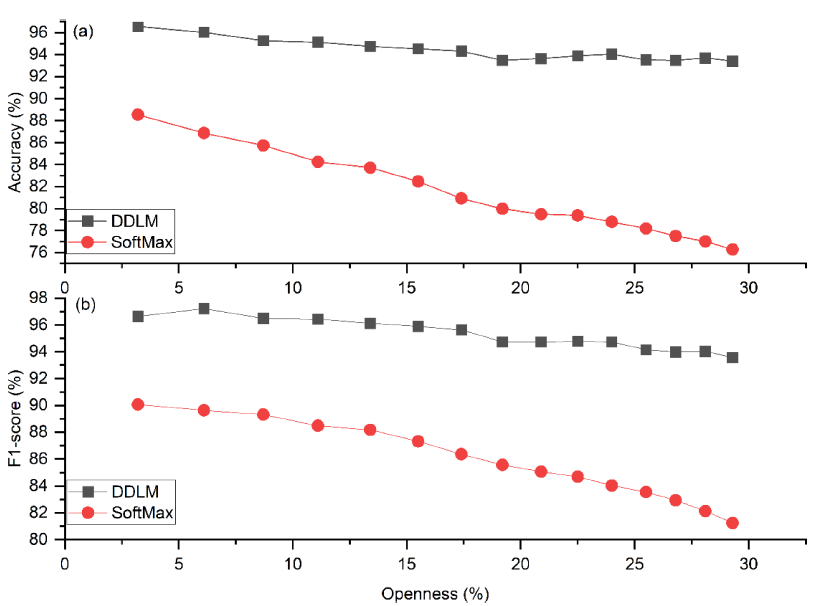
\includegraphics[width=\linewidth]{./img/ddlm_openness.png}
\end{center}
\caption{開放性による精度とF1スコアの変化}
\end{figure}

また,DDLMとソフトマックスのみを用いた手法による比較の混同行列を図7, 8に示します.

\begin{figure}[H]
\begin{center}
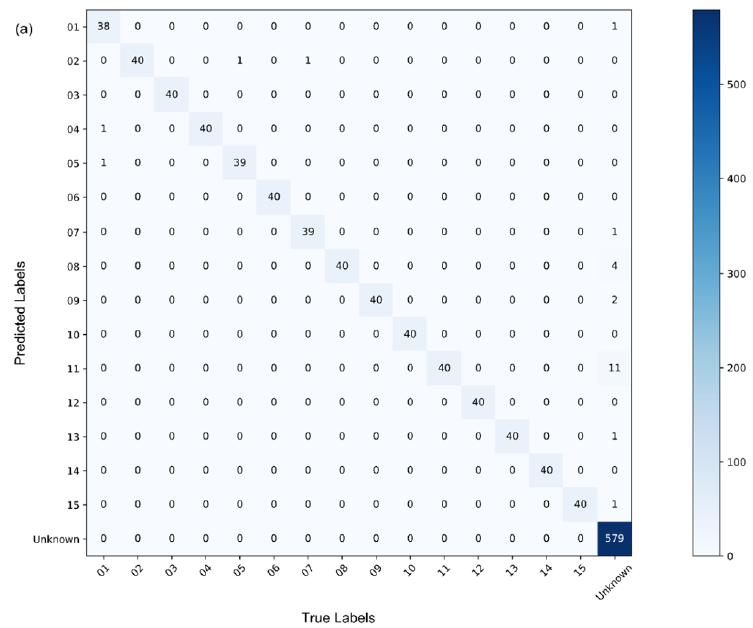
\includegraphics[width=0.7\linewidth]{./img/ddlm_conf.png}
\end{center}
\caption{DDLMを用いた場合の混同行列}
\end{figure}

\begin{figure}[H]
\begin{center}
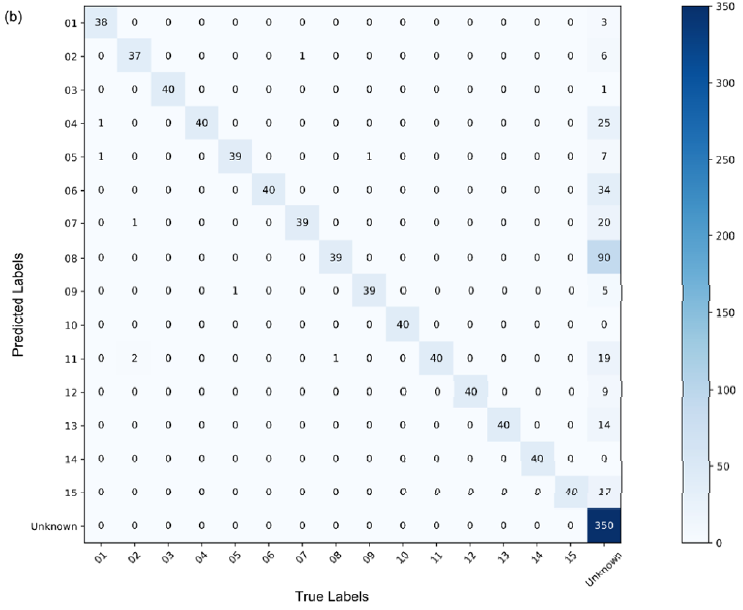
\includegraphics[width=0.7\linewidth]{./img/softmax_conf.png}
\end{center}
\caption{ソフトマックスを用いた場合の混同行列}
\end{figure}

図7, 8の比較から,DDLMはopennessが最も高い場合に平均精度93.57\%, F1スコア93.42\%を達成し,従来のソフトマックス法とのパフォーマンスギャップは精度で17.14\%, F1スコアで12.32\%まで開くことが確認できます.

    \item クローズドセットの場合

先ほどまでのオープンセットの場合と異なり,クローズドセットの場合には,表3に示すように平均99\%の精度を達成しており,提案手法が高いロバスト性を備えていることが分かります.

\begin{figure}[H]
    \caption*{表3: クローズドセットの場合,被験者の増加に伴う精度とF1スコアの変化}
    \begin{center}
    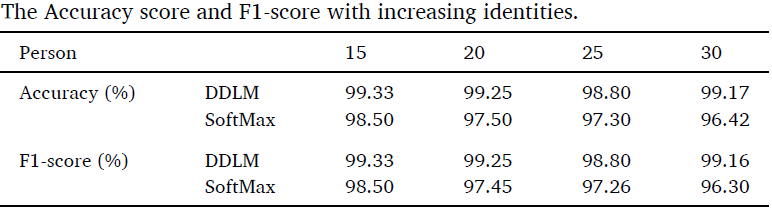
\includegraphics[width=0.8\linewidth]{./img/result_closed.png}
    \end{center}
    \end{figure}
\end{itemize}

\subsection{呼吸に基づく人間のidentification}
\begin{itemize}
    \item 『Human Identification by Measuring Respiration Patterns Using Vital FMCW Radar\cite{respi}』
\end{itemize}

\subsubsection{提案法}
本論文は,24GHz FMCWレーダを使用して呼吸パターンを測定する人間識別の方法を提案しています.レーダで得たデータは従来法のKNN(k-nearest neighbor)法の代わりに,3つの隠れ層を持つ多層パーセプトロンで処理され,ソフトマックス層で分類されます.KNN法は多クラス分類のためのシンプルで効果的な手法だが,本論文が注目する深層学習アルゴリズムと比較すると精度が劣ります.

提案されるアルゴリズムでは,
\begin{enumerate}
    \item 受信したビート信号の高速フーリエ変換結果を用いて,複数ターゲットの距離パラメータを求める
    \item 距離指標のバイタルドップラー信号を用いてDNN(Deep Neural Network)で処理する.図9にネットワークのアーキテクチャを示します.
    \begin{enumerate}
        \item まずLMS(Least Mean Squared)フィルタに通し,SN比の改善を行う.
        \item 入力は隠れ層で処理されていき,各層は全結合層で構成される.
        \item 出力層ではソフトマックスでユーザ推定を行う.
        フィルタ処理された信号行列$R$は適応フィルタの結果を表し,DNNの出力は$H$で表され,次のように表されます.
\begin{equation}\label{}
    H = \sigma(W_k^T ... \sigma(W_2^T \sigma(W_1^T R)))
    \end{equation}
    ここで,$W_k$は$k$番目の重み行列$(k=1, 2, ..., K)$,$T$は転地,()はReLUなどの活性化関数を表している.
\end{enumerate}
\end{enumerate}

\begin{figure}[H]
    \begin{center}
    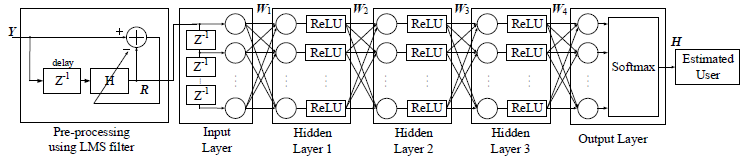
\includegraphics[width=0.9\linewidth]{./img/proposed_dnn.png}
    \end{center}
    \caption{提案されたDNNのアーキテクチャ}
\end{figure}

3つの隠れ層を使用すると,任意の決定協会を有利活性化関数で表すことができます.この関数はあらゆるタイプの滑らかななマッピングをあらゆる精度で近似でき,追加の層はより複雑な表現を学習できます.本論文において,レイヤーを増やしても$(K>3)$,大幅な精度の向上は達成されず,ただトレーニングにかかる時間は長くなりました.

\subsubsection{実験}
実験は韓国のDGISTの室内で行われたました.この実験では,ターゲットからの距離推定結果から選択されたターゲットのバイタルドップラー信号を求めました.本論文に記載されている4人の被験者は異なるバイタルドップラー信号を生成しました.これらを図10に示します.

\begin{figure}[H]
\begin{center}
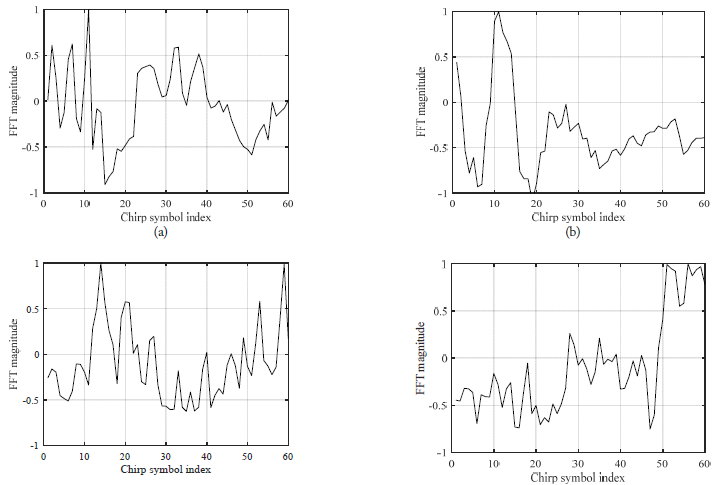
\includegraphics[width=\linewidth]{./img/doppler_signal.png}
\end{center}
\caption{4人の被験者のドップラー信号}
\end{figure}

レーダシステムの視野が$\pm$15°以内なので,同時に計測できる人数は2人です.したがって核実験における人々の間の距離は2mに設定されました.提案したアルゴリズムの改善を実証するために表4に結果の表を示しました.

\begin{figure}[H]
\caption*{表4: KNNベースのアルゴリズムと提案されたアルゴリズムの分類精度}
\begin{center}
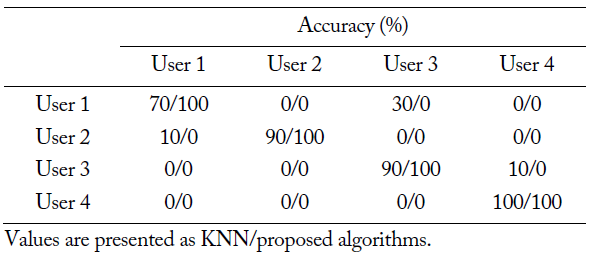
\includegraphics[width=0.8\linewidth]{./img/knn_proposed.png}
\end{center}
\end{figure}

表4はKNNベースのアルゴリズムと提案されたアルゴリズムの分類精度を示し,比較しています.
ユーザを分類するために使用されるDNNは,サイズ1×60の入力層,サイズ60×500の第一隠れ層,サイズ500×250の第二隠れ層,サイズ250×500の第三隠れ層,350×4の出力層で構成されています.DNNベースの識別結果は,KNNベースの識別結果よりも優れていることが確認できます.

\subsection{歩行特徴に基づく人間のidentification}
\begin{itemize}
    \item 『Indoor Person Identification Using a Low-Power FMCW Radar\cite{MD}』
\end{itemize}

\subsubsection{概要}
低出力レーダから取得したマイクロドップラー(MD)シグネチャを使用して,歩行特性に基づいて一連の人物を識別する方法を調査します.そのために,深い畳み込みニューラルネットワークに基づくロバストな特徴学習アプローチを提案します.人々は2つの異なる部屋を自由に歩き回ることができ,使用した5人のターゲットの検証セットで24.70\%,テストセットで21.54\%の分類エラー率を達成しました.

\subsection{人間の行動のclassification}
\begin{itemize}
    \item 『Classification of Human Activities based on Automotive Radar Spectral Images Using Machine Learning Techniques: A Case Study\cite{motion}』
\end{itemize}

\subsubsection{概要}
本論文では,車載レーダから取得したマイクロドップラースペクトル画像からスタートし,Human Activities Recognitionの3つの異なる方法を提示し,それらの長所・短所を説明します.3つの方法は,CNN, PCA, MDマップからのパラメータ抽出です.人の歩行速度に関連する3種の活動を含むデータセットのケーススタディを検討している.実験結果から,適切なパラメータ選択により,計算コストが比較的小さく,94\%を超える精度を達成できると分かりました.これは,より複雑なフレームワークで達成される精度よりも高くなります.

\section{計画}
\begin{itemize}
    \item 『Indoor Person Identification Using a Low-Power FMCW Radar』と『Classification of Human Activities based on Automotive Radar Spectral Images Using Machine Learning Techniques: A Case Study』の続きを読み込む
    \item 他の論文もサーベイし,卒研に活かせる部分を発見する
\end{itemize}

\begin{thebibliography}{}
    \item{pointcloud} Zhao, Peijun, et al. "Human tracking and identification through a millimeter wave radar." Ad Hoc Networks 116 (2021): 102475.
    \item{DDLM} Yan, Baiju, et al. "Heart signatures: Open-set person identification based on cardiac radar signals." Biomedical Signal Processing and Control 72 (2022): 103306.
    \item{respi} Kim, Sangdong, et al. "Human Identification by Measuring Respiration Patterns Using Vital FMCW Radar." Journal of Electromagnetic Engineering and Science 20.4 (2020): 302-306. 
    \item{MD} Vandersmissen, Baptist, et al. "Indoor person identification using a low-power FMCW radar." IEEE Transactions on Geoscience and Remote Sensing 56.7 (2018): 3941-3952.
    \item{motion} Senigagliesi, Linda, et al. "Classification of Human Activities based on Automotive Radar Spectral Images Using Machine Learning Techniques: A Case Study." 2022 IEEE Radar Conference (RadarConf22). IEEE, 2022.
\end{thebibliography}
\end{document}